\documentclass[tikz]{standalone}
% https://tex.stackexchange.com/questions/31708/draw-a-bivariate-normal-distribution-in-tikz

\usepackage{amsmath}
\usepackage{physics}
\usepackage{pgfplots}

\let\Re\undefined
\let\Im\undefined
\DeclareMathOperator{\Re}{\operatorname{Re}}
\DeclareMathOperator{\Im}{\operatorname{Im}}

\pgfplotsset{compat=1.17}

\begin{document}
	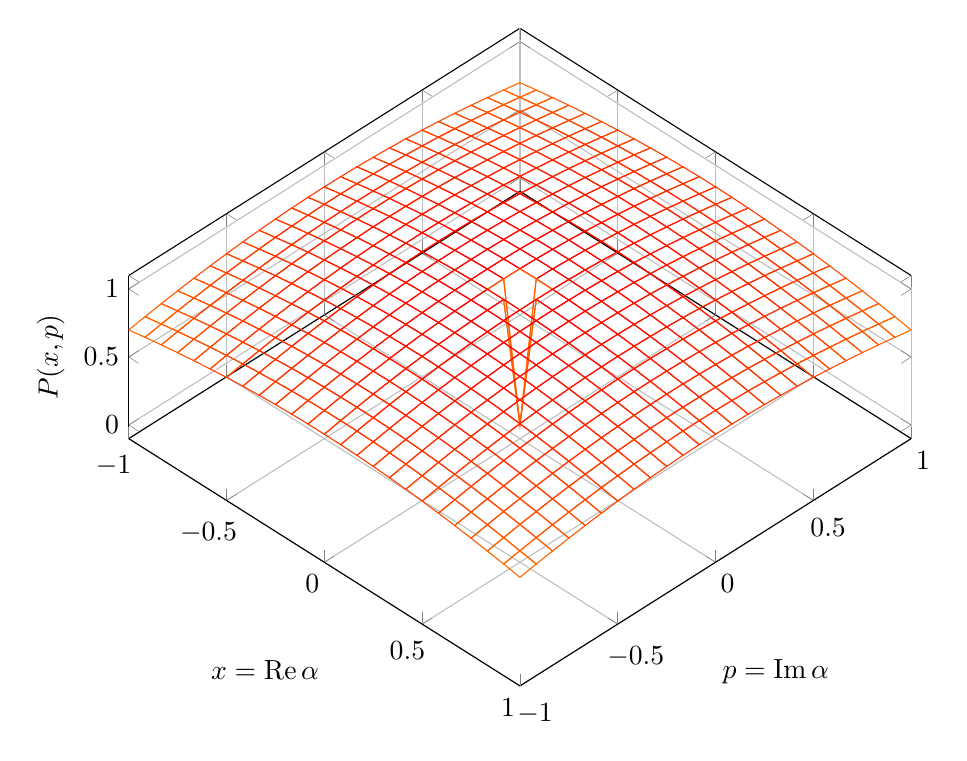
\begin{tikzpicture}
		\begin{axis}[
			cycle list name=exotic,
		    xlabel={$x=\Re{\alpha}$},
		    ylabel={$p=\Im{\alpha}$},
		    zlabel={$P(x,p)$},
		    width=0.95\linewidth,
		    view={45}{65},
		    grid=major,
		    domain=-1:1,
		    y domain=-1:1,
		]
			\addplot3[
				mesh,
%				samples=50,
%			    domain=-8:8,
			]{sin(deg(sqrt(x^2+y^2)))/sqrt(x^2+y^2)};
		\end{axis}
	\end{tikzpicture}
\end{document}